\chapter{Planificación}

La planificación en el desarrollo de un proyecto es un aspecto clave para organizar las tareas, trabajar de manera eficiente y garantizar el cumplimiento de plazos y objetivos. En este capítulo se detallará el enfoque elegido para el desarrollo del proyecto, la distribución de las tareas y los costes asociados al desarrollo completo.

\section{Desarrollo ágil}
El desarrollo ágil promueve un enfoque flexible y adaptativo para la gestión de proyectos, especialmente en la creación de software. Entre otros, se caracterizan por iteraciones cortas, aceptación del cambio en los requisitos durante el desarrollo y entregas continuas de producto (con el objetivo de satisfacer al cliente con software de valor desde el inicio)\cite{agileprinciples}.

\textit{Kanban} es un sistema de gestión del flujo de trabajo. Utiliza un tablero con columnas que representan diferentes etapas del proceso (como el trabajo realizado, lo que está en proceso y tareas futuras). Los elementos del proyecto se mueven a lo largo del tablero; esto facilita al desarrollador trabajar de acuerdo al enfoque de Kanban: el desarrollador debe centrarse en limitar las tareas en progreso para mejorar la productividad y evitar la sobrecarga\cite{majkamastering}.

Se ha optado por \textbf{Kanban} por su flexibilidad y simplicidad. Permite gestionar el proyecto sin imponer plazos fijos, algo útil cuando se trabaja de forma individual y se necesita adaptar el ritmo entorno a la carga de trabajo y resolución de problemas. Kanban, al facilitar la priorización de tareas y la realización de entregas funcionales frecuentes, permite avanzar poniendo el foco en conseguir las metas (hitos) establecidos.

Existen herramientas de gestión de proyectos que nos facilitan seguir un desarrollo con este enfoque, como \textit{Trello}\footnote{\url{https://trello.com/es}} o \textit{Click Up}\footnote{\url{https://clickup.com/es-ES}}, con tableros personalizados y colaborativos para organizar tareas de proyectos.


\section{Distribución de tareas}
Siguiendo el enfoque \textit{Kanban}, se ha establecido un \textbf{tablero} (como se puede ver en la Figura \ref{fig:tablero_kanban}) con las tareas a realizar en el proyecto, que incluirán (entre otras) la implementación de funcionalidades, resolución de problemas encontrados y realización de pruebas. El progreso en su desarrollo se identifica por la posición de la tarjeta en el tablero (por ejemplo: pendiente, en proceso o terminada) .

De esta forma, en el desarrollo de un conjunto de tareas, cuando éstas suponen un momento importante del desarrollo, se relaciona al milestone (definición de milestones en el capítulo de análisis \ref{sec:milestones}) como marcador de dicho logro. Por tanto, los milestones (aún sujetos a cambios según las necesidades) guían la planificación del proyecto y permiten el seguimiento temporal del mismo.
\begin{figure}[ht!]
    \centering
    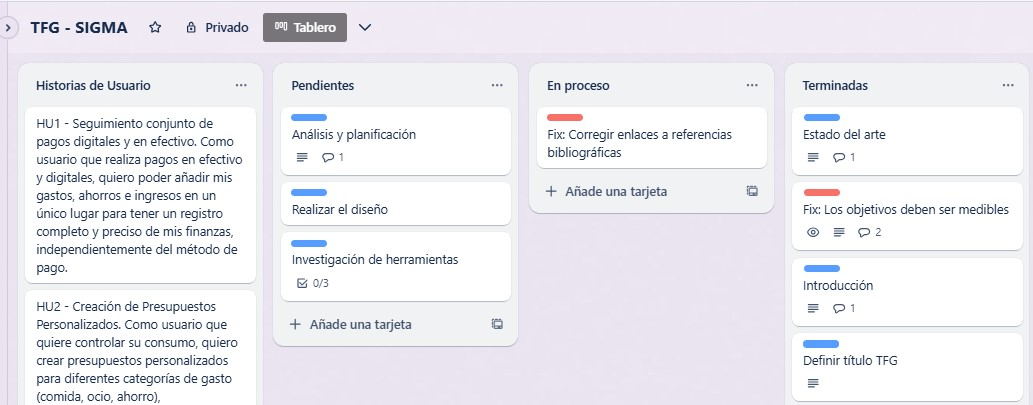
\includegraphics[width=\linewidth]{imagenes/tablero_kanban.jpg}
    \caption{Captura de pantalla del tablero kanban en \textit{Trello}.}
    \label{fig:tablero_kanban}
\end{figure}


\section{Costes}
En este capítulo se describen los recursos y materiales usados en el desarrollo del proyecto, junto con los costos asociados a cada uno de ellos.

\subsection{Recursos humanos}

En el desarrollo de la aplicación web \textit{SIGMA}, se ha contado con un desarrollador que ha hecho también las labores de diseño para la interfaz y redacción de este documento.

\subsection{Hardware y software}
Como recursos materiales, han sido utilizados un ordenador personal portátil y un monitor (Tabla \ref{tab:coste-total}),
propiedad del desarrollador, los cuales han sido de gran utilidad para las tareas de diseño y desarrollo al permitir el visionado de diferentes recursos simultáneamente.

\begin{table}[H]
    \begin{center}
    \begin{tabular}{| l | c | c | c |}
        \hline
        \textbf{Entidad} & \textbf{Precio original} \\ \hline
        % Desarrollador & 3.757,81\euro \\
        % Diseñador  & 284,06\euro \\ \hline
        Hardware & 721,68\euro \\ \hline
        \textbf{Coste total}: & \textbf{721,68\euro} \\ \hline
    \end{tabular}
    \caption{Coste total}
    \label{tab:coste-total}
    \end{center}
\end{table} 

Para desarrollar este proyecto no se ha usado ningún software ni biblioteca de pago con el propósito de reducir costes, por lo que el software externo no incrementa el coste total. Por otro lado, el coste del hardware anteriormente mencionado, viene condicionado por la vida útil estimada de los dispositivos. En el caso de un ordenador portátil y un monitor, se estiman entre 5 y 7 años. La tasa de amortización corresponde a la fórmula: 100/vida útil, de esta manera se establece la tasa de amoritización del hardware en un 20\% anual\cite{fleet_amortizacion_ordenadores}\cite{holded_amortizacion_equipos}.
\begin{equation}
    \textbf{Cuota Amortización Anual} = \frac {\text{Coste Hardware}}{\text{5 años}} = \text{144,336 €/año}
\end{equation}

\begin{equation}
    \textbf{Cuota Amortización Mensual} = \frac {\text{Cuota Amortización Anual}}{\text{12 meses}} = \text{12,03 €/mes}
\end{equation}

\begin{equation}
    \textbf{Cuota en 8 meses de desarrollo} =\text{12,03 €/mes} \times \text{8 meses} = \text{96,224 €}
\end{equation}

\subsection{Presupuesto sobre profesionales implicados}
En esta sección se detallarán los costos del proyecto entorno al salario del desarrollador que lo contruye. Se considerará el perfil de un puesto junior de desarrollador \textit{fullstack}, cuyo salario anual oscila entre los 17.000€ y 22.000€ \cite{glassdoor2024}.
Teniendo en cuenta que el desarrollo ha tomado un tiempo aproximado de 460 horas, se puede calcular un coste estimado del salario del desarrollador, el cual se detalla a continuación:

\begin{equation}
    \textbf{Salario medio fullstack junior} =  \frac {\text{19.500 €/año} }{ \text{12 meses}} = \text{1.625 €/mes}
\end{equation}

El salario por hora se calcula dividiendo el salario mensual entre 160 horas, que es el promedio de horas laborales al mes:

\begin{equation}
    \textbf{Salario por hora} = \frac {\text{1.625 €/mes}}{160 \text{ horas}} = \text{10,16 €/hora}
\end{equation}

Teniendo en cuenta las 460 horas de trabajo, se puede calcular el coste total del salario:

\begin{equation}
    \textbf{Coste total salario} = \text{460 horas} \times \text{10.16 €/hora} = \text{4.876 €}
\end{equation}

% Para el diseño, se tendrá en cuenta el perfil de un diseñador gráfico, cuyo salario medio es de unos 18.180 € \cite{glassdoor-dis-grafico-2024}. Teniendo en cuenta que el diseño ha supuesto un aproximado de 30 horas. Partiendo de esta información, se puede calcular el coste total del salario del diseñador, el cual se detalla a continuación:

% \begin{equation}
%     \textbf{Salario medio diseñador gráfico} =  \frac {\text{18.180 €/año} }{ \text{12 meses}} = \text{1,515 €/mes}
% \end{equation}

% El salario por hora se calcula dividiendo el salario mensual entre 160 horas, que es el promedio de horas laborales al mes:

% \begin{equation}
%     \textbf{Salario por hora} = \frac {\text{1,515 €/mes}}{160 \text{ horas}} = \text{9,47 €/hora}
% \end{equation}

% Teniendo en cuenta las 30 horas de trabajo, se puede calcular el coste total del salario del diseñador:

% \begin{equation}
%     \textbf{Coste salario} = \text{30 horas} \times \text{9,47 €/hora} = \text{284,06 €}
% \end{equation}

\subsection*{Total}

Sumando los costes asociados a los salarios y materiales usados, se obtiene el coste total aproximado del proyecto (representado en la Tabla \ref{tab:coste-total}).

\begin{table}[H]
    \begin{center}
    \begin{tabular}{| l | c | c | c |}
        \hline
        \textbf{Entidad} & \textbf{Coste } \\ \hline
        Desarrollador & 4.876\euro \\
        % Diseñador  & 284,06\euro \\ \hline
        Hardware & 96,224\euro \\ \hline
        \textbf{Coste total}: & \textbf{4.972,22\euro} \\ \hline
    \end{tabular}
    \caption{Coste total.}
    \label{tab:coste-total}
    \end{center}
\end{table} 